\chapter{实验细节}

\section{实验目标}
本次实验的目标是构建一个小型领域知识图谱，提取中山大学教师信息中的实体和关系，并将其导入到Neo4j数据库中进行可视化和分析。

\section{方法实现}
\subsection{数据来源与预处理}
\begin{itemize}
    \item 数据来源于中山大学官网的教师个人主页。
    \item 使用Python脚本对原始数据进行清洗和预处理，生成结构化的CSV文件。
\end{itemize}

\subsection{NLP工具的使用}
\begin{itemize}
    \item 使用spaCy工具进行分词、命名实体识别（NER）和关系抽取。
    \item 提取的实体包括教师姓名、工作单位（学院）和所属大学。
    \item 提取的关系包括“工作于”和“隶属于”。
\end{itemize}

\subsection{Neo4j图谱构建}
\begin{itemize}
    \item 使用py2neo库连接Neo4j数据库。
    \item 将提取的实体和关系以JSON格式存储，并通过脚本将其导入Neo4j数据库。
    \item 在Neo4j中创建节点和边，节点包括Person、Organization和University，边包括WORKS\_AT和BELONGS\_TO。
\end{itemize}


\section{数据统计}
\subsection{原始数据统计}
原始数据包含中山大学中国语言文学系的教师信息，数据来源于官网教师个人主页。以下是原始数据的统计信息：
\begin{itemize}
    \item 教师总人数：12608
    \item 涉及的学院：88
    \item 所属大学：1所（中山大学）
\end{itemize}

\subsection{知识图谱统计}
基于原始数据构建的知识图谱包含以下点和边的数量：
\begin{itemize}
    \item 节点总数：12608个Person节点，88个Organization节点，1个University节点，总计12697个节点。
    \item 边总数：12608条WORKS\_AT关系，88条BELONGS\_TO关系，总计12796条边。
    \begin{itemize}
        \item WORKS\_AT关系：12608条（每个教师与其学院的关系）。
        \item BELONGS\_TO关系：88条（学院与大学的关系）。
    \end{itemize}
\end{itemize}

\subsection{统计说明}

相关数据保存在 data 文件夹中，包含爬虫原数据、清洗后的数据以及导入neo4j的JSON文件。

\section{实验内容}
\subsection{原始文本片段}
\begin{lstlisting}[style=cleanpython]
**丁文俊**

中国语言文学系, 文艺学教研室 副教授

丁文俊，男，广东东莞人，1988年生，文学博士，中山大学中国语言文学系副教授，硕士生导师。在中山大学中国语言文学系获得文学学士学位（2012.6）；在华东师范大学中国语言文学系文艺学专业师从朱国华教授，先后获得文学硕士学位（2015.6）和文学博士学位（2019.6）；2016年10月—2018年7月，获国家留学基金委资助，前往法国国立东方语言文化学院( Institut National des Langues et Civilisations Orientales )访学；2019年9月—2025年4月，在中山大学中国语言文学系师从王坤教授，从事科研博士后和专职科研岗工作。  

主要研究方向为文艺社会学，研究领域涵盖西方马克思主义美学、文化研究和晚明美学。

一、代表性研究成果  
[西方文论方向]  
[1] 丁文俊：《阿多诺美学的自然记忆与“感性......
  
二、科研项目  
[1] 2023年国家社科基金后期资助项目“记忆的政治：‘阿本之争’的历史境......

三、联系方式  
邮箱：dingwj7@mail.sysu.edu.cn

\end{lstlisting}

\subsection{提取的实体与关系}
\begin{itemize}
    \item 实体：
    \begin{itemize}
        \item Person: 丁文俊
        \item Organization: 中国语言文学系
        \item University: 中山大学
    \end{itemize}
    \item 关系：
    \begin{itemize}
        \item 丁文俊 WORKS\_AT 中国语言文学系
        \item 中国语言文学系 BELONGS\_TO 中山大学
    \end{itemize}
\end{itemize}

\section{实验结果与分析}
\subsection{图谱覆盖范围}
图谱包含了中山大学中国语言文学系的所有教师信息及其与学院、大学的关系。

\subsection{准确性分析}
实体和关系提取的准确率较高，但对于部分复杂描述可能存在漏提或误提的情况。


\section{核心代码及说明}
以下是实验中使用的部分核心代码：
\begin{lstlisting}[style=cleanpython]
def extract_information(description):
    nlp = spacy.load("zh_core_web_sm")
    doc = nlp(description)

    # Extract name
    name_match = re.search(r"\*\*(.*?)\*\*", description)
    name = name_match.group(1) if name_match else ""

    # Extract workplace and department
    workplace = ""
    department = ""
    for ent in doc.ents:
        if ent.label_ == "ORG":
            if "大学" in ent.text:
                workplace = ent.text
            else:
                department = ent.text

    return {
        "name": name,
        "workplace": workplace,
        "department": department
    }
\end{lstlisting}

上述代码实现了从教师信息描述中提取核心实体（姓名、工作单位、部门）的功能：
\begin{itemize}
    \item 使用spaCy加载中文语言模型进行分词和命名实体识别。
    \item 使用正则表达式提取教师姓名。
    \item 遍历命名实体，识别出工作单位和部门。
\end{itemize}

\section{算法处理介绍}
本实验的算法处理流程如下：
\begin{enumerate}
    \item **数据预处理**：对原始文本数据进行清洗，去除无关信息，确保数据格式统一。
    \item **实体提取**：使用spaCy进行命名实体识别，提取教师姓名、工作单位和所属大学。
    \item **关系抽取**：基于规则和上下文，提取教师与工作单位、工作单位与大学之间的关系。
    \item **数据存储**：将提取的实体和关系以JSON格式存储，便于后续导入Neo4j。
    \item **图谱构建**：使用py2neo库将JSON数据导入Neo4j，创建节点和边，构建知识图谱。
\end{enumerate}

\section{结果展示}
\subsection{关系图展示}
由于图谱较大，对于硬件要求较高，以下展示部分关键节点和关系的可视化结果：

\begin{figure}[htbp]
    \centering
    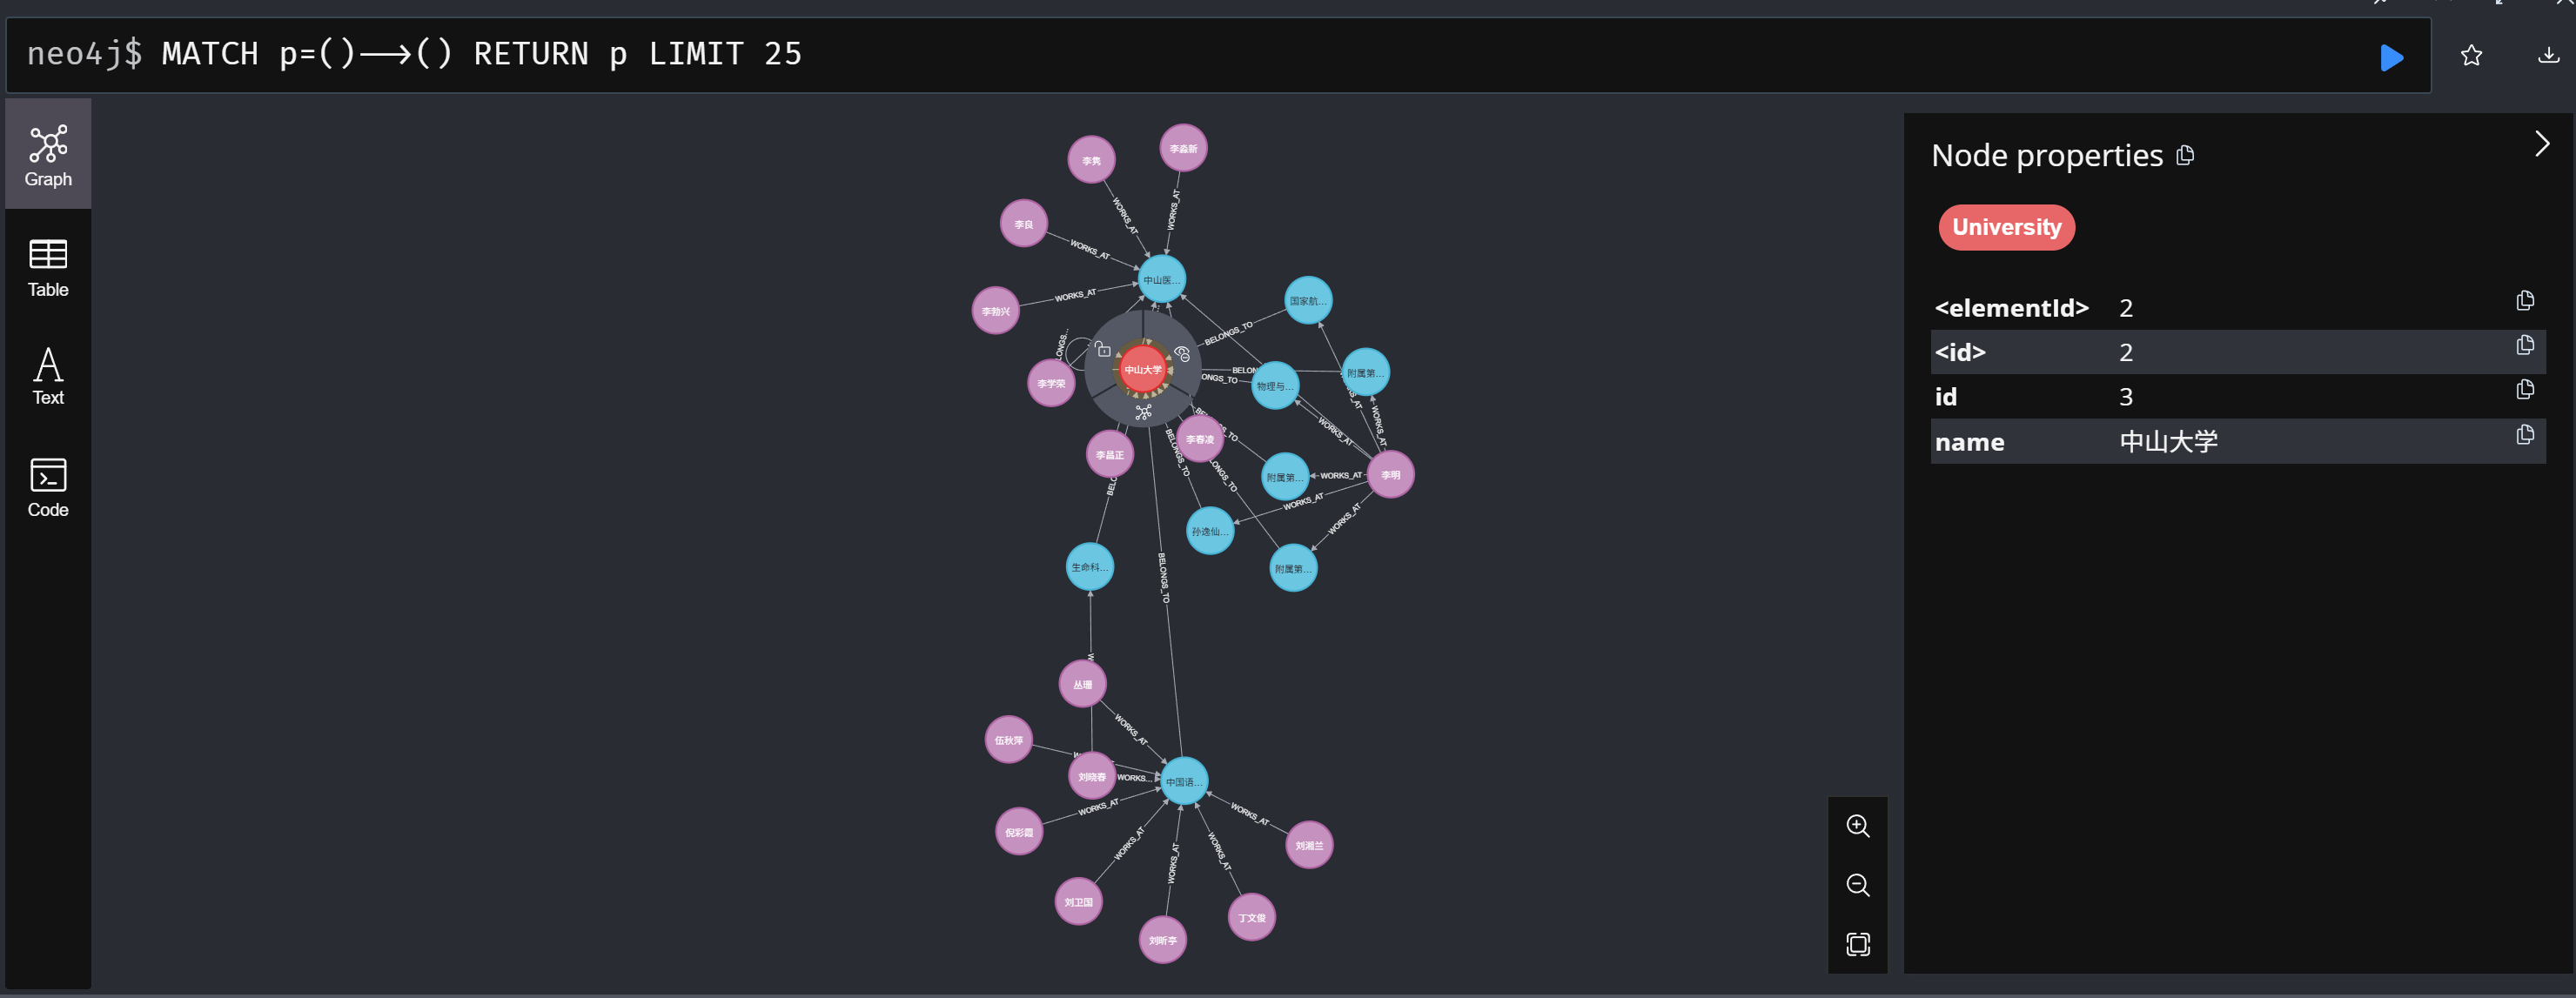
\includegraphics[width=\textwidth]{image/result1.png}
    \caption{完整的关系图}
\end{figure}

\subsection{学校与各学院的关系图}
\begin{figure}[htbp]
    \centering
    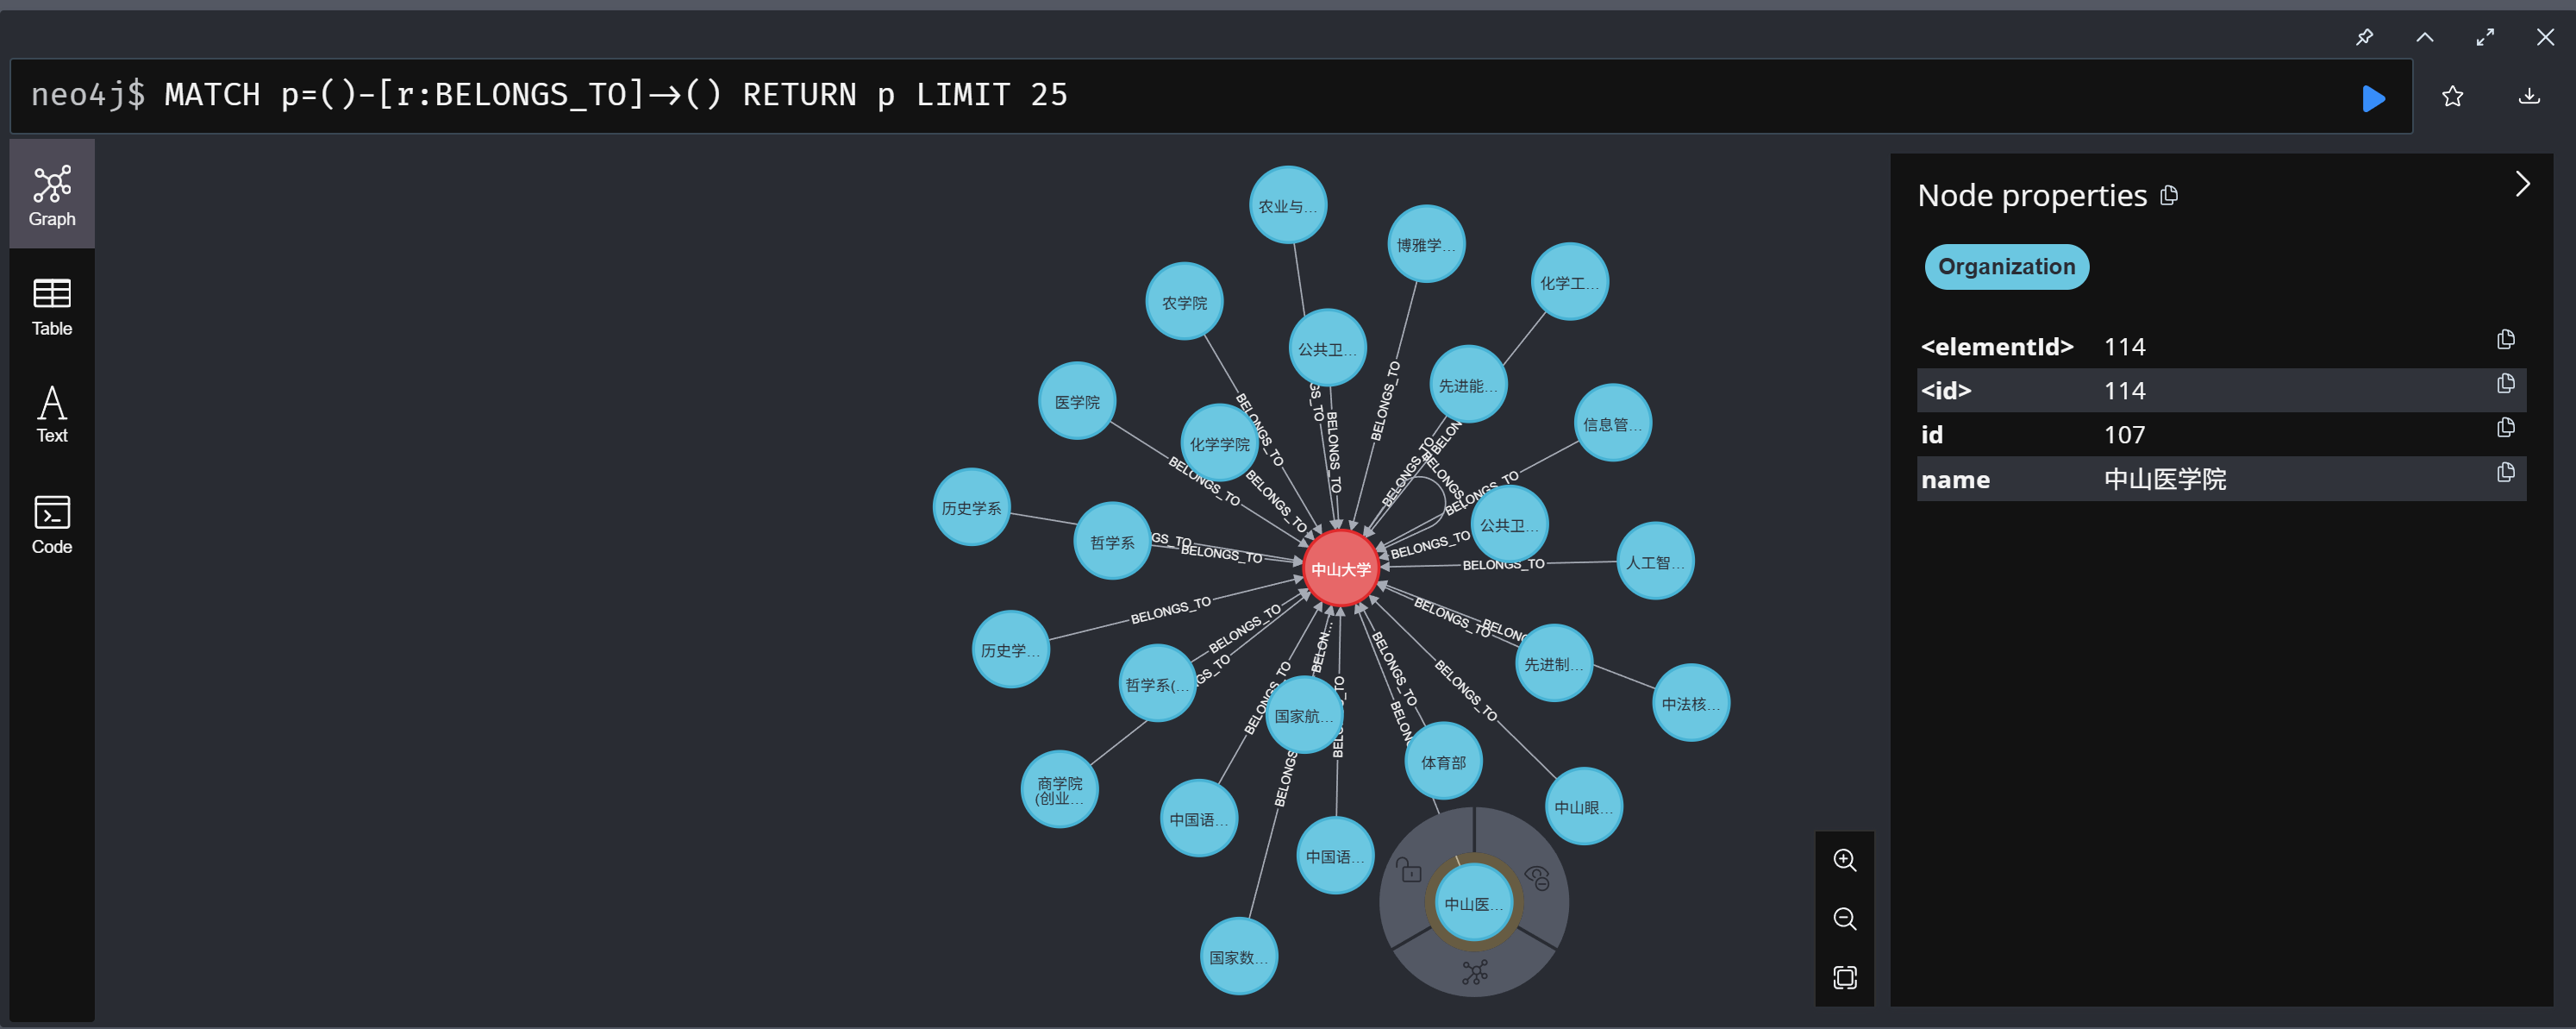
\includegraphics[width=\textwidth]{image/result3.png}
    \caption{学校与各学院的关系图}
\end{figure}

\subsection{各学院与老师的关系图}
\begin{figure}[htbp]
    \centering
    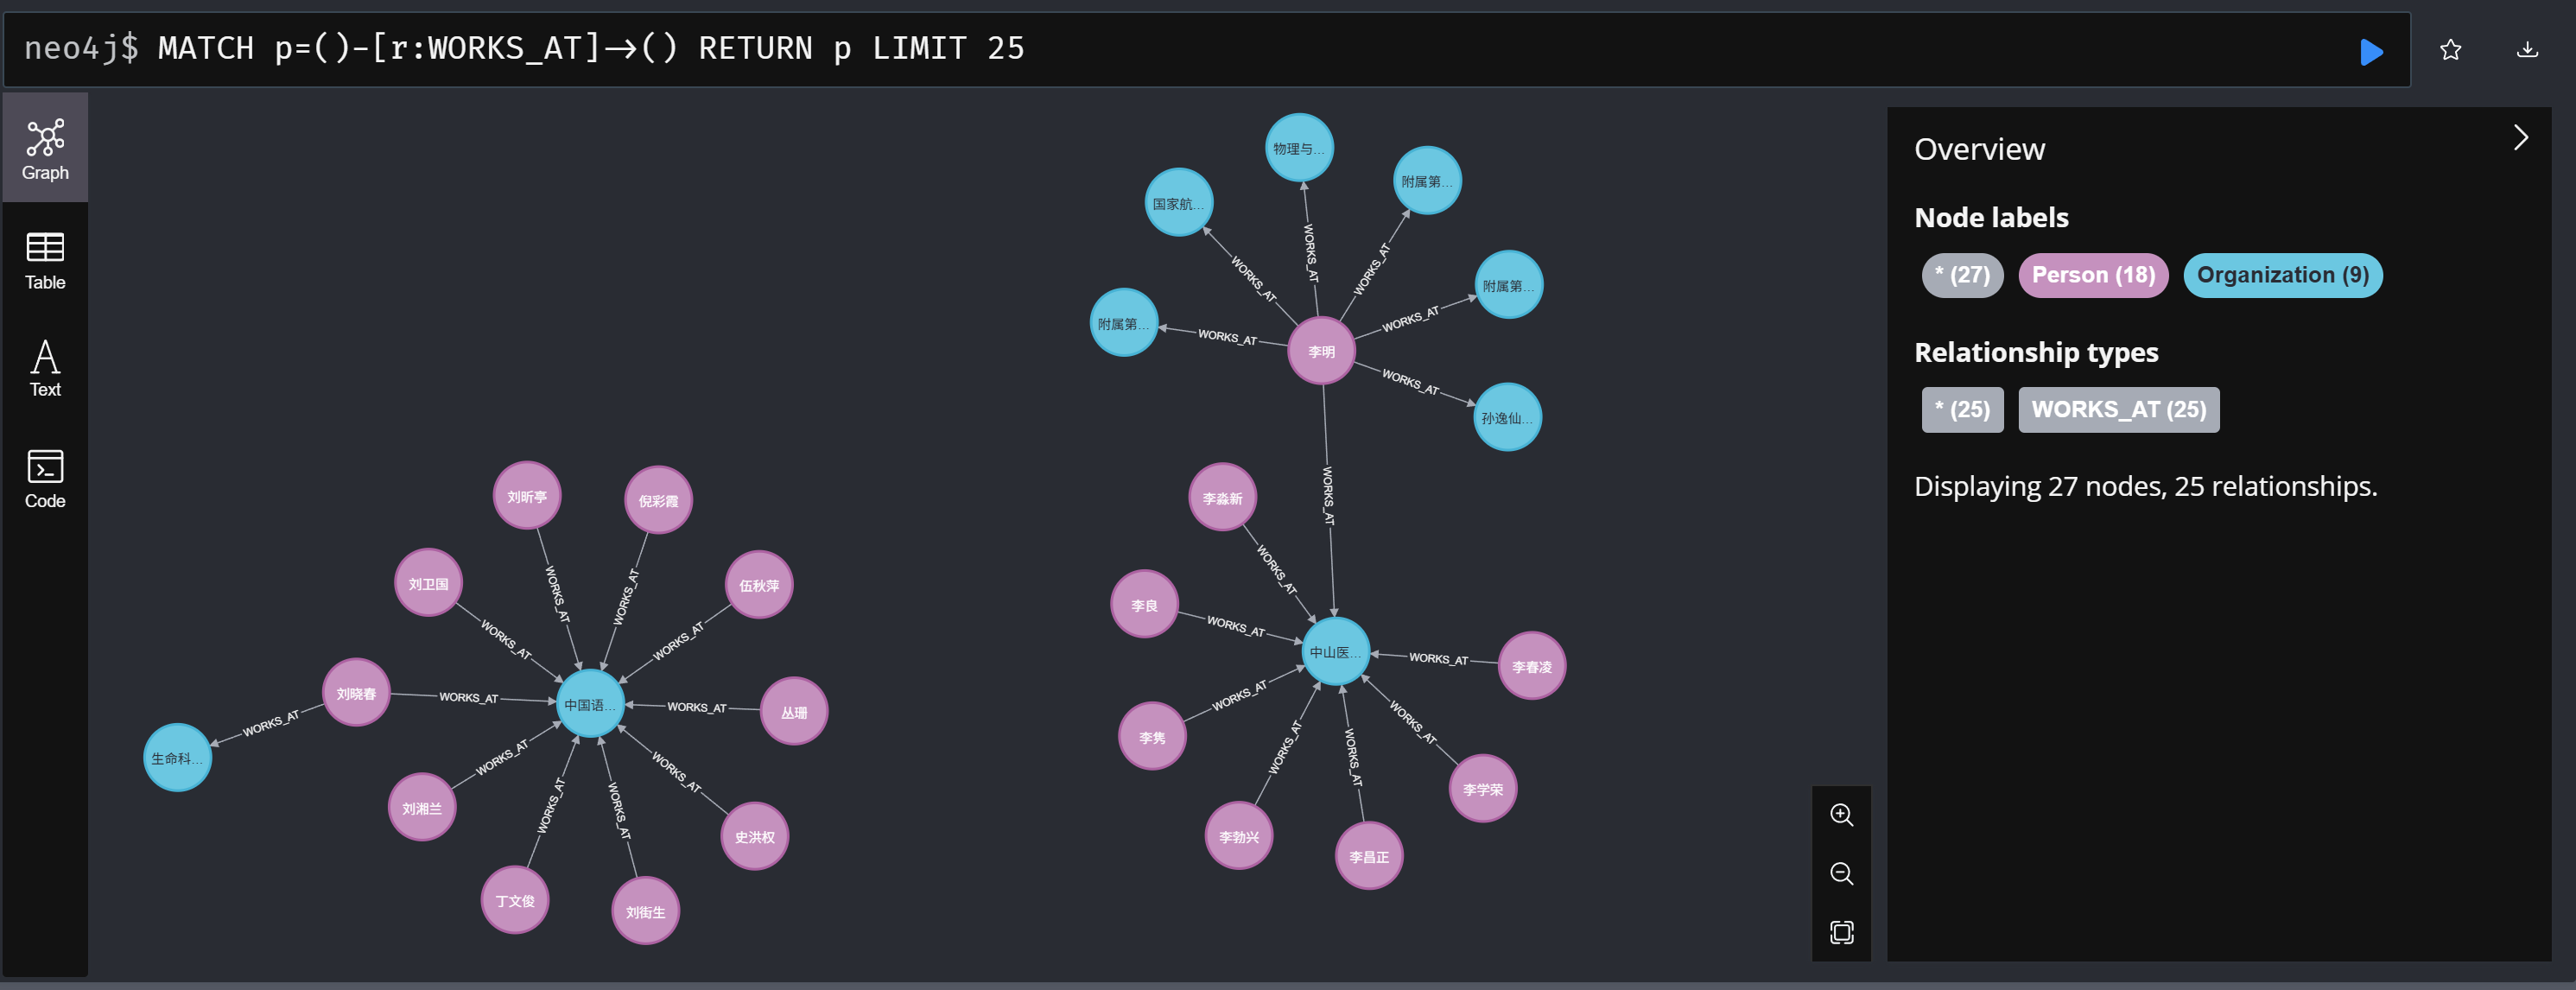
\includegraphics[width=\textwidth]{image/result2.png}
    \caption{各学院与老师的关系图}
\end{figure}

\chapter{总结}

本次实验完成了从文本到图谱的端到端流程验证，证明了利用现有 NLP 工具与图数据库可以快速构建中小规模的知识图谱，后续可在抽取质量和图谱分析深度上继续增强。

\section{实验总结}
本次实验旨在构建中山大学教师信息的小型领域知识图谱，通过网页采集、文本清洗、命名实体识别与关系抽取，最终将提取结果导入 Neo4j 并完成可视化展示。实验验证了基于规则与现成 NLP 工具（spaCy）在结构化基础信息抽取任务中的实用性，能够较为稳定地抽取出教师姓名、工作单位与学院-学校层级关系，并以图数据库形式呈现节点与关系。

\section{主要成果}
\begin{itemize}
    \item 成功采集并清洗了目标学院的教师简介文本，生成了用于抽取的原始语料和结构化 CSV/JSON 文件；
    \item 基于 spaCy 与简单规则实现了实体（Person、Organization、University）的识别，以及 WORKS\_AT、BELONGS\_TO 等关系的抽取；
    \item 使用 py2neo 将抽取结果批量导入 Neo4j，构建了可交互的知识图谱，并在报告中给出多张可视化截图以展示图谱结构与关键节点；
    \item 给出了核心代码片段、Cypher 查询示例与数据存储格式，具备基本复现性。
\end{itemize}
